% !TeX root = ../main.tex

\section{Data} \label{sec: data}
This chapter will describe the empirical landscape of commodity markets and available data. Section \ref{subsec: data_commodity classification and selection} addresses the reasons for the specific choice of commodity classes examined. Sections \ref{subsec: data_source market} and \ref{subsec: data_target market} describe the data used for the source and target market respectively. 

\subsection{Commodity Classification \& Selection} \label{subsec: data_commodity classification and selection}
\subsection{Source Market: Global Benchmark Exchanges} \label{subsec: data_source market}

\vspace{-10pt}
\begin{table}[h!]
\caption{Possible Source Data Sources/Series}
\label{tab:target-data-sources}
\footnotesize

\begin{tabularx}{\textwidth}{
    @{}
    >{\raggedright\arraybackslash}p{0.24\textwidth}
    >{\raggedright\arraybackslash}p{0.08\textwidth}
    >{\raggedright\arraybackslash}X
    >{\raggedright\arraybackslash}p{0.10\textwidth}
    @{}
}
\toprule
\textbf{Source} &
\textbf{Freq.} &
\textbf{Commodities} &
\textbf{Dates} \\
\midrule
Yahoo Finance (quoted from COMEX, NY Mercantile, CBOT, CME, ICE Futures) &
Daily &
Gold, Silver, Copper, Crude Oil WTI, Crude Oil Brent, Natural Gas, Corn, Oats, Wheat, Rough Rice, Soybeans, Feeder Cattle, Lean Hogs, Live Cattle, Cocoa, Coffee, Cotton, Lumber, Orange Juice, Sugar &
1999-2026 \\
\bottomrule
\end{tabularx}
\end{table}



\vspace{-10pt}
\begin{figure}[htbp]
    \caption{Example figure with two subfigures.}
    \centering

    \setlength{\figsep}{4mm}
    \setlength{\subfigwidth}{\dimexpr(\linewidth-\figsep)/2\relax}

    \setkeys{Gin}{width=\subfigwidth}

    \begin{tikzpicture}[
        picnode/.style={inner sep=0pt},
        node distance=4mm and \figsep,
        subcap/.style={below=0mm of #1, text width=\subfigwidth, align=center, inner sep=0pt}
    ]

        \node[picnode] (A) {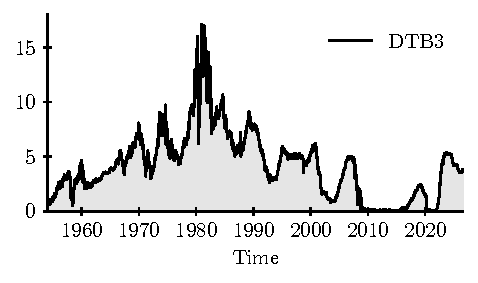
\includegraphics{1.5_figures/test figures/dtb3.pdf}};
        \node[right=of A, picnode] (B) {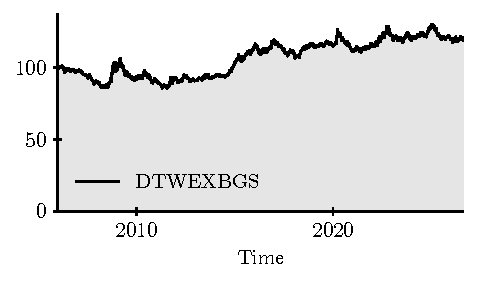
\includegraphics{1.5_figures/test figures/dtwexbgs.pdf}};
        \node[below=of A, picnode] (C) {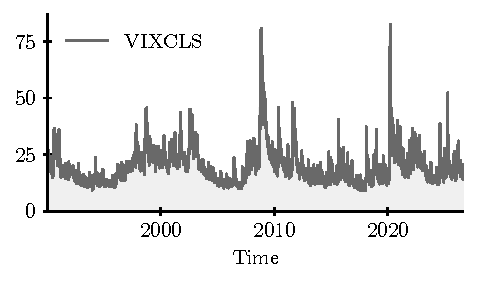
\includegraphics{1.5_figures/test figures/vixcls.pdf}};
        \node[right=of C, picnode] (D) {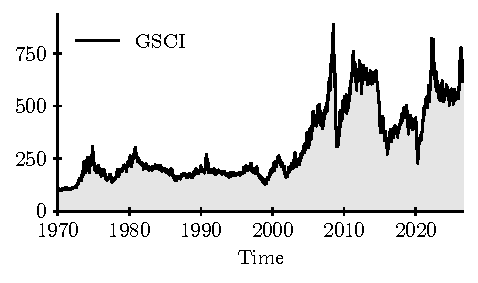
\includegraphics{1.5_figures/test figures/gsci.pdf}};


        \node[subcap=A] {\subcaption{DTB3}\label{fig:example-a}};
        \node[subcap=B] {\subcaption{DTWEXBGS}\label{fig:example-b}};

    \end{tikzpicture}

    \label{fig:example}
\end{figure}
\vspace{-10pt}
\subsection{Target Markets: Data-Sparse Economies}  \label{subsec: data_target market}

\vspace{-10pt}
\begin{table}[h!]
\caption{Possible Target Data Sources/Series}
\label{tab:target-data-sources}
\footnotesize

\begin{tabularx}{\textwidth}{
    @{}
    >{\raggedright\arraybackslash}p{0.24\textwidth}
    >{\raggedright\arraybackslash}p{0.08\textwidth}
    >{\raggedright\arraybackslash}X
    >{\raggedright\arraybackslash}p{0.10\textwidth}
    @{}
}
\toprule
\textbf{Source} &
\textbf{Freq.} &
\textbf{Commodities} &
\textbf{Dates} \\
\midrule
\href{http://www.dce.com.cn/dceg/channel/list/468.html}{DCE (Dalian Commodity Exchange)} &
Daily &
No. 1 Soybean, No. 2 Soybean, Soybean Meal, Soybean Oil,
RBD Palm Olein, Corn, Corn Starch, Pol RG Rice, Egg, Live Hogs,
Fiberboard, Blockboard, Log, Coking Coal, Coke, Iron Ore,
LLDPE, LLDPE MAF, PVC, PVC MAF, Polypropylene,
Polypropylene MAF, Ethylene Glycol, Ethenylbenzene, LPG,
Benzene &
2006-2026 \\
\midrule
\href{https://english.czce.com.cn/en/MarketData/HistoricalData/H081002017index_1.htm}{Zhengdong Commodity Exchange} &
Daily &
Apple, Cotton, Chinese Jujube, Cotton Yarn, Flat Glass, Japonica Rice, Late Rice, Methanol, Rapeseed Oil, Polyester Staple Fiber, Wheat PM, Early Rice, Rapeseed Meal, Rapeseed, Soda Ash, Ferrosilicon, Manganese Silicon, White Sugar, PTA, Urea, Wheat WH, Thermal Coal, Peanut Kernel, Paraxylene, Sodium Hydroxide, Polyethylene Terephthalate Resin for Bottles, Propylene &
2015-2026 \\
\midrule
\href{https://www.mcxindia.com/market-data/historical-data}{Multi Commodity Exchange (MCX) India} &
Daily &
Aluminium, Cardamom, Copper, Cotton, Cotton Oil, Crude Oil, ELECDMBL, Gold, Goldguinea, Goldm, Goldpetal, Goldten, Kapas, Lead, Leadmini, MCXBULLDEX, MCXMETLDEX, Metha Oil, Natural Gas Mini, Natural Gas, Nickel, Silver, Silver 100, Silver M, Silver MIC, Steel Rebar, Zinc, Zinc Mini&
2003-2026 \\
\bottomrule
\end{tabularx}
\end{table}



\subsection{Feature Engineering}    \label{subsec: data_feature engineering}
\subsection{Descriptive Statistics \& Stylised Facts}   \label{subsec: data_descriptive statistics}
\subsection{Train/Validation/Test Split}    \label{subsec: data_train validation test split}
